
\subsection{External calibration feasibility, index use, and recovery}
Every external partition recovers all 360 calibration messages. Stable-cover fraction varies by partition, while all 7,000 covers are exercised in the complete 30-session schedule for every seed. Tables~\ref{tab:calibration} and~\ref{tab:indexuse} report the frozen external results.

\begin{table}[t]
\caption{External Caltech-101 calibration results under the frozen protocol.}
\label{tab:calibration}
\small
\begin{tabular}{r l r r r r}
\toprule
Seed & Projection & Stable covers & Stable frac. & Recovery & Max RS\\
\midrule
11 & random\_04 & 4,184 & 0.598 & 360/360 & 5\\
29 & random\_04 & 3,795 & 0.542 & 360/360 & 37\\
47 & random\_15 & 4,756 & 0.679 & 360/360 & 0\\
71 & random\_20 & 3,933 & 0.562 & 360/360 & 11\\
101 & random\_28 & 4,167 & 0.595 & 360/360 & 0\\
\midrule
All & -- & -- & 0.595 mean & 1,800/1,800 & 37\\
\bottomrule
\end{tabular}
\end{table}

\begin{table}[t]
\caption{External index-use diagnostics over the complete 30-session schedule. Every partition exercises all 7,000 available covers.}
\label{tab:indexuse}
\small
\begin{tabular}{rrrrrr}
\toprule
Seed & Unique covers & Min freq. & Mean freq. & Max freq. & Frequency CV\\
\midrule
11&7,000&3&11.471&21&0.2307\\
29&7,000&4&11.471&20&0.2299\\
47&7,000&3&11.471&21&0.2295\\
71&7,000&4&11.471&21&0.2307\\
101&7,000&4&11.471&21&0.2276\\
\bottomrule
\end{tabular}
\end{table}

\begin{figure}[t]
\centering
\begin{minipage}[t]{.46\textwidth}
\centering
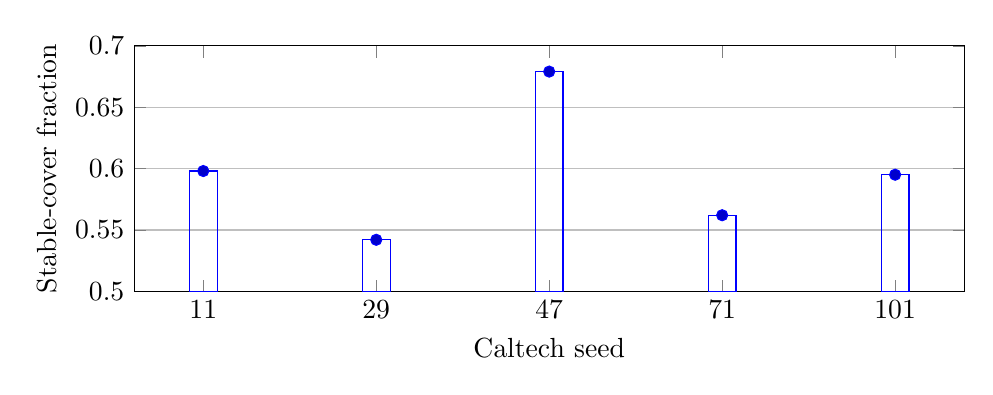
\begin{tikzpicture}
\begin{axis}[width=\linewidth,height=4.7cm,ymin=.50,ymax=.70,xtick={1,2,3,4,5},xticklabels={11,29,47,71,101},xlabel={Caltech seed},ylabel={Stable-cover fraction},ymajorgrids=true]
\addplot+[ybar] coordinates {(1,.598)(2,.542)(3,.679)(4,.562)(5,.595)};
\end{axis}
\end{tikzpicture}
\end{minipage}\hfill
\begin{minipage}[t]{.46\textwidth}
\centering
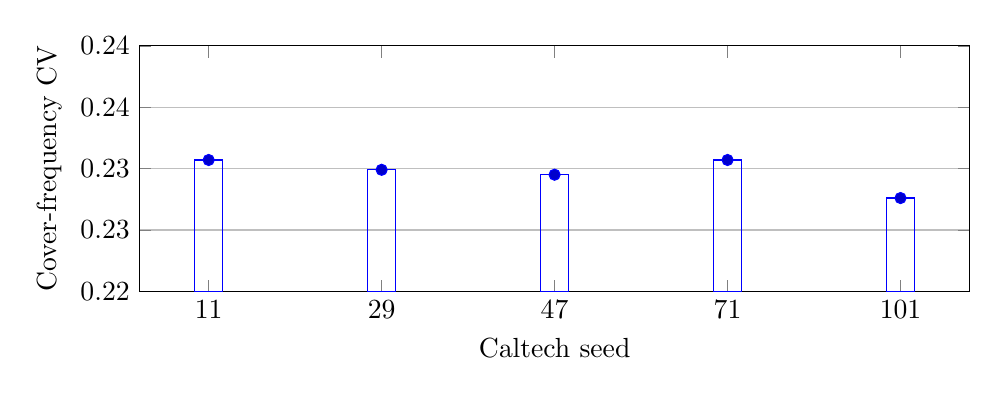
\begin{tikzpicture}
\begin{axis}[width=\linewidth,height=4.7cm,ymin=.22,ymax=.24,xtick={1,2,3,4,5},xticklabels={11,29,47,71,101},xlabel={Caltech seed},ylabel={Cover-frequency CV},ymajorgrids=true]
\addplot+[ybar] coordinates {(1,.2307)(2,.2299)(3,.2295)(4,.2307)(5,.2276)};
\end{axis}
\end{tikzpicture}
\end{minipage}
\caption{External calibration diagnostics. Stable-cover fractions vary by partition, while complete-schedule cover-use dispersion remains tightly clustered.}
\Description{Two bar charts across the five Caltech seeds: stable-cover fractions range from 0.542 to 0.679; cover-frequency coefficients of variation remain near 0.23.}
\label{fig:caldiag}
\end{figure}

\subsection{Unseen holdout robustness}
The external holdout campaign recovers 1,163 of 1,200 authenticated messages (96.92\%). The 37 unsuccessful trials are concentrated in the unseen 12\% central crop, which reaches the Reed--Solomon correction radius of 64 bytes. Each of the other seven transformations recovers 150/150 messages. Crop 8\% lowers mean cover-label accuracy to 0.707, yet group majority and RS128 preserve all 150 authenticated messages; rotate 9 degrees similarly reaches mean label accuracy 0.860 while retaining full message recovery.

\begin{table}[t]
\caption{External holdout results. Cover-label accuracy is measured before group majority and FEC; message success requires final authenticated plaintext recovery.}
\label{tab:holdout}
\small
\begin{tabular}{lrrrr}
\toprule
Holdout transformation & Auth. recovery & Mean label acc. & Min label acc. & Max RS\\
\midrule
Gaussian $\sigma=9$&150/150&0.964&0.941&0\\
Gaussian $\sigma=15$&150/150&0.950&0.911&2\\
Blur 1.2&150/150&0.958&0.902&0\\
Blur 1.8&150/150&0.928&0.844&5\\
Crop 8\%&150/150&0.707&0.641&34\\
Crop 12\%&113/150&0.603&0.525&64\\
Rotate $5^\circ$&150/150&0.923&0.896&0\\
Rotate $9^\circ$&150/150&0.860&0.806&26\\
\midrule
All holdouts&1,163/1,200&--&--&64\\
\bottomrule
\end{tabular}
\end{table}

Per-partition authenticated success is 240/240, 214/240, 240/240, 231/240, and 238/240 for seeds 11, 29, 47, 71, and 101. Maximum RS corrections are 55, 64, 37, 64, and 63 respectively.

\begin{figure}[t]
\centering
\begin{tikzpicture}
\begin{axis}[width=.9\textwidth,height=5.6cm,ymin=.5,ymax=1.03,xtick=data,xticklabels={G9,G15,B1.2,B1.8,C8,C12,R5,R9},xlabel={Holdout transformation},ylabel={Rate / accuracy},legend style={at={(0.5,1.03)},anchor=south,legend columns=2},ymajorgrids=true]
\addplot+[mark=*] coordinates {(1,1)(2,1)(3,1)(4,1)(5,1)(6,.7533)(7,1)(8,1)};
